\chapter{Design Motivation and Overview}
\label{ch:fdsp-apa-design}

%%%%%%%%%%%%%%%%%%%%%%%%%%%%%%%%%%%%%%%%%%%%%%%%%%%%%%%%%%%%%%%%%%%%
\section{Introduction to Single-Phase Far Detector in DUNE}
\label{sec:fdsp-design-intro}

The DUNE \dword{spmod} will be the culmination of several decades
of \lartpc technology development, and once operational, it will open new windows of opportunity in the study
of neutrinos.  DUNE's rich physics program, with discovery
potential for \dword{cpv} in the neutrino sector, and capability to make
significant observations of nucleon decay and astrophysical events, is enabled
by the exquisite resolution of the \lartpc detector technique.

Experience with design, construction, operation, and data
analysis with numerous single-phase \lartpc experiments and prototypes has informed the approach to
realizing the massive DUNE \dwords{spmod}. Each far \dword{detmodule} will feature the largest \lartpc{}s ever
constructed, at approximately \nominalmodsize active volume each.  Aside from the
challenges inherit in such a large undertaking, DUNE presents the added complication of construction and operation in a location
that is one mile underground with limited access.

The design of the DUNE \dword{spmod} that is presented in this document
reflects an approach to achieve the science goals of the experiment, and
address the challenges of constructing and operating a massive detector in a deep
underground environment.


%%%%%%%%%%%%%%%%%%%%%%%%%%%%%%%%%%%%
\section{Single-Phase \lartpc Operational Principle}
\label{sec:fdsp-design-op}

The precision tracking and calorimetry offered by the single-phase \lartpc
technology provides excellent ability to identify interactions of interest
while mitigating sources of background.  The operational principle of a
single-phase \lartpc is summarized here for reference.

Charged particles traversing the active volume of the \lartpc ionize the medium,
while also producing scintillation light.  The ionization drifts along
an \efield that is present throughout the volume, towards a series of
anode layers.  Each anode layer is composed of finely spaced wires arranged at
characteristic angles, and appropriate biasing of these wires allows the
ionization to drift through the successive layers before terminating on a wire
in the Collection layer.  The individual wires in the anode layers can be
instrumented with low-noise electronics that record the current in the wire as
a function of time.  The argon scintillation light, which at \SI{128}{nm} wavelength
is deep in the UV spectrum, can be recorded by photon detectors that shift the
wavelength closer to the visible spectrum and subsequently record the time and
pulse characteristics of the incident light.

%\begin{dunefigure}[\lartpc Single-Phase Operational
 %   Principle]{fig:design_lartpcdiagram}{A diagram depicting the operational   principle of a single-phase \lartpc.  Ionization produced in the TPC will  drift towards the anode, creating signals in the wires that are recorded   by readout electronics.  Scintillation light produced in the TPC can be   captured and recorded by photon detectors integrated into the anode  structure.}
%\includegraphics[width=0.4\textwidth]{lartpc_diagram.jpg}
%\end{dunefigure}

%\fixme{Include diagram of basic single-phase \lartpc operational principle.  Expand previous paragraph.}

The performance of the \lartpc hinges on several key factors.  First, the
purity of the liquid argon must be extremely high in order for ionization to
be able to drift over several meters towards the anode planes.  The levels of
electronegative contaminants (e.g., oxygen, water), must be reduced and
maintained to \dword{ppt} levels in order to achieve minimum charge attenuation
over the longest drift lengths in the \lartpc.   Second, the electronic readout
of the \lartpc requires very low noise levels so that the signal of drifting
ionization is clearly discernible over the baseline of the electronics.  
Third, a uniform \efield must be established over the detector volume, requiring a robust and stable high voltage system.  Finally, the sheer size of the \dword{spmod} means that once it is filled with \lar, all components within the cryostat are inaccessible for decades.  All internal devices must have long operating lifetimes at \lar temperatures.

%%%%%%%%%%%%%%%%%%%%%%%%%%%%%%%%%%%
\section{Motivation of Single-Phase \lartpc Design at DUNE}
\label{sec:fdsp-design-impl}

The DUNE Single-Phase Far Detector builds on several decades of experience in designing, constructing, and operating \lartpc{}s.  It implements unique design features to maximize the capability of the experiment, as well as new features motivated by the unprecedented scale of the Far Detector modules and the deep underground location where construction will occur.

Among the features driven by the underground location of the experiment, all detector components are sized to fit within the constraints of the \surf shafts and access pathways.

A drift time of several milliseconds is typical for ionization to arrive at the anode wires after drifting several meters.  This lengthy duration of time, as well as aspects of the DUNE physics program looking for rare and low-energy processes, makes the deep underground location essential for the \dword{spmod}.  The  $\sim$\SI{1.5}{km} overburden of earth greatly reduces the rate of cosmic rays reaching the active volume of the \dword{spmod}, greatly enhancing the ability to search for rare and low-energy signatures without the influence of cosmic-induced backgrounds.  


%%%%%%%%%%%%%%%%%%%%%%%%%%%%%%%%%%%%%%%%%%%%%%%%%%%%%%%%%%%%%%%%%%%%
\section{Overview of the Single-Phase Design}
\label{sec:fdsp-ov-model}

The DUNE \dword{spmod} features a \nominalmodsize active mass \lartpc, with all associated cryogenic, electronic readout, computing, and safety systems.  The \dword{spmod} is designed to maximize the active volume within the confines of the membrane cryostat while minimizing dead regions.  The detector elements have been modularized such that their production can proceed in parallel with the construction of the DUNE caverns and cryostats, and sized so that they conform to the access restrictions for transport underground.  Table~\ref{tab:dune-sp-parameters} summarizes some of the high-level parameters of the \dword{spmod}.

\begin{dunetable}[\dword{spmod} parameters]{lll}{tab:dune-sp-parameters}{\dword{spmod} parameters}
Parameter & Value & Note \\ \toprowrule
Cryostat \lar mass & \larmass & \\ \colhline 
Active \lar mass & \nominalmodsize & \\ \colhline 
Active Height & \tpcheight & \\ \colhline 
Active Length & \sptpclen & \\ \colhline 
Maximum Drift & \spmaxdrift & \\ \colhline 
%Number of \dwords{apa} & 150 & \\ 
%Number of \dwords{cpa} & XXX & \\ 
%Number of \dword{pd}s & XXX & \\ \colhline
Number of \dword{apa} channels & \spnumch & \\\colhline 
Number of \dword{pds} channels & \spnumpdch & \\ 
\end{dunetable}

%\fixme{Fix all numbers in previous table.  Pls use/fix values in def.tex. -Anne}

The cryostat is constructed such that its long axis is aligned with the beam arriving from \fnal.  The TPC  inside the cryostat is composed of two rows of \dwords{cpa} oriented along the long axis of the cryostat, flanked on either side by rows of \dwords{apa}.  A \dword{fc} completely surrounds the four
open sides of the four drift regions to ensure that the \efield within is uniform and unaffected by the presence of the cryostat walls and other nearby conductive structures.  Integrated within each \dword{apa} are elements of the \dword{pds} as well as electronics to process the \dword{apa} signals.  Around the periphery of the TPC various instrumentation for monitoring the cryogenic environment is present.  Outside of the cryostat, additional electronic readout and data acquisition equipment is present to transfer information from the \dword{detmodule}.  Figure~\ref{fig:dune-sp-overview} illustrates the basic arrangement of the TPC elements within the \dword{spmod}.

\begin{dunefigure}[DUNE \dword{spmod} diagram]{fig:dune-sp-overview}{A diagram showing the arrangement of the main TPC elements in the \dword{spmod}.  Two rows of \dwords{cpa} are interleaved with three rows of \dwords{apa}.  The \dword{fc} structure (only partially depicted to enable visibility of other elements) surrounds the outer area of the \dword{apa} and \dword{cpa} rows.  Elements of the \dword{pds} are integrated within the \dword{apa} structure.}
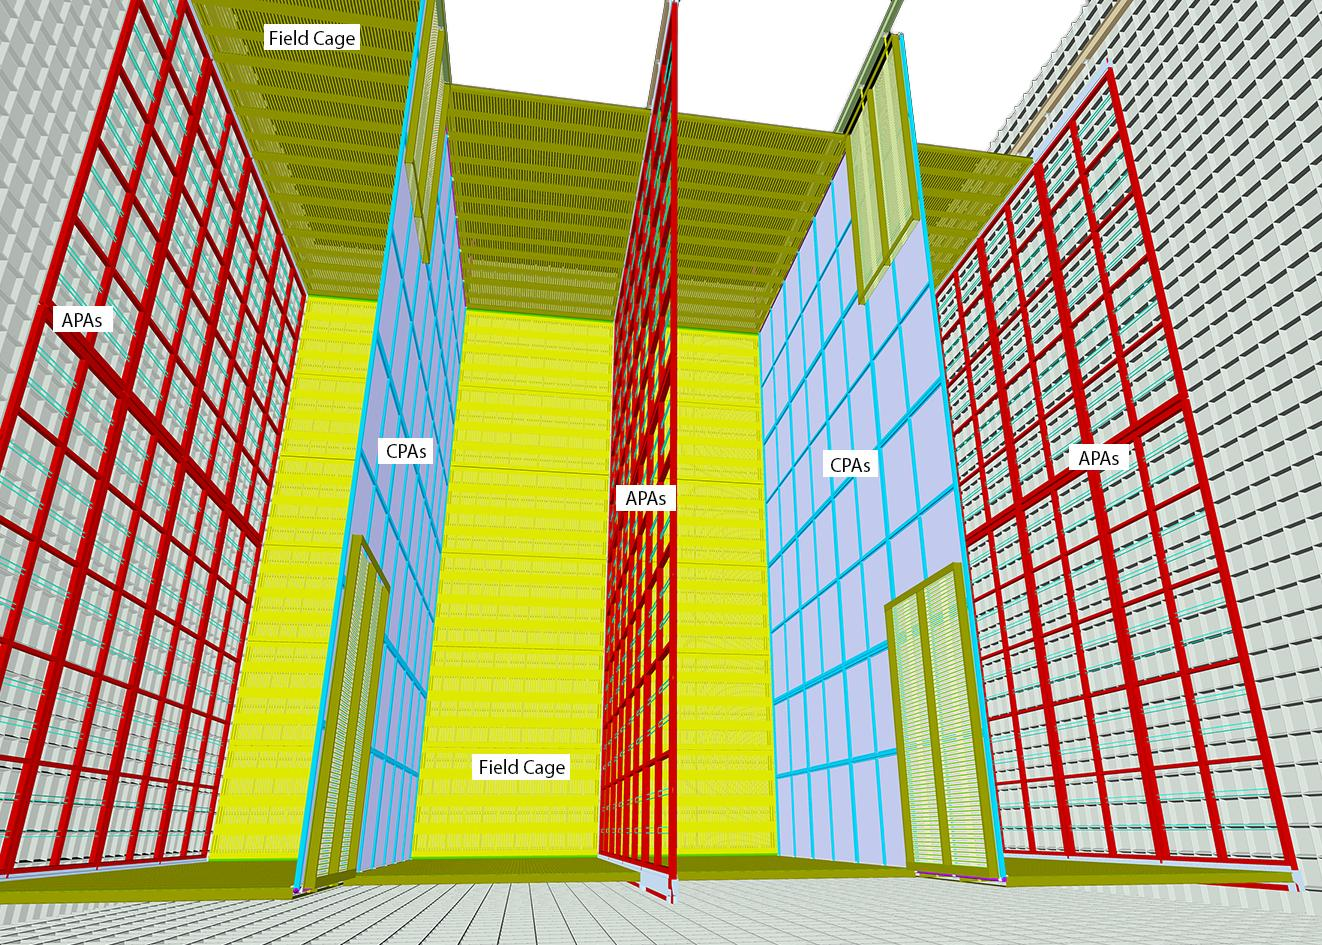
\includegraphics[width=0.6\linewidth]{DUNE-SP.jpg}
\end{dunefigure}



%%%%%%%%%%%%%%%%%%%%%%%%%%%%%%%%%%%%%%%%%%%%%%%%%%%%%%%%%%%%%%%%%%%%
\section{Detector Systems}
\label{sec:fdsp-ov-sys}


%The elements composing the DUNE-SP detector module include the time projection chamber (TPC), the cold electronics (\dword{ce}), and the photon detection system (\dword{pds}).  The TPC components, e.g., anode planes, cathode planes and the field cage, are designed in a modular way.  
%The six \dwords{apa} are arranged into two \dword{apa} planes, each consisting of three side-by-side \dwords{apa}. Between them,  
%a central cathode plane, composed of 18 \dword{cpa} modules, splits the TPC volume into two electron-drift regions, one on each side of the cathode plane. 
 
%\begin{itemize}
%\item{\dword{apa} - Anode Plane Assemblies.}
%\item{\dword{hv} - High Voltage system.  This system is composed of the Cathode Plane Arrays (\dwords{cpa}), Field Cage (\dword{fc}), and \dword{hv} feedthrough.}
%\item{Electronics}
%\item{\dword{pd} - Photon Detection System}
%\item{\dword{daq} - Data Acquisition System}
%\item{CISC - Cryogenic Instrumentation and Slow Controls}
%\end{itemize}


Table~\ref{tab:tpc-systems} lists the principal detection systems of the \dword{spmod} along with the primary purpose of each system.  In this section, the primary detector systems are introduced briefly.  The subsequent chapters of this document provide extensive descriptions of each of these systems. 

\begin{dunetable}[\dword{spmod} systems]{lll}{tab:tpc-systems}{\dword{spmod} systems.}
System & Name  & Purpose   \\  \toprowrule
\hyperref[ch:fdsp-apa]{\dshort{apa}}  & anode plane assemblies & ionization signal development \\ \colhline
\hyperref[ch:fdsp-hv]{\dshort{hv}} & high voltage & establish uniform drift field \\ \colhline
\hyperref[ch:fdsp-tpc-elec]{\dshort{ce}} & cold electronics & process \dword{apa} signals  \\ \colhline
\hyperref[ch:fdsp-pd]{\dshort{pd}} & photon detection & light collection and triggering\\ \colhline
\hyperref[ch:fdsp-daq]{\dshort{daq}} & data acquisition & record and handle digital data \\ \colhline
\hyperref[ch:fdsp-slow-cryo]{\dshort{cisc}} & cryogenics instrumentation and slow controls & Maintain and monitor \lar volume\\ 
\end{dunetable}

%\begin{dunetable}[Single-Phase Far Detector TPC components, dimensions and
%    quantities]{lll}{tab:tpc-components}{Single-Phase Far Detector TPC components, dimensions and quantities}
%Detection Element & Approx Dimensions  & Quantity   \\  \toprowrule
%\hyperref{ch:fdsp-apa}{\dword{apa}}  & 6~m H by 2.4~m W  & 50  per anode plane, 150 total  \\  \colhline
%\dword{cpa} module  & 2~m H by 1.2~m W  & 6 per \dword{cpa} column,   \\  
%  &  & 300 total  \\  \colhline
% Top \dword{fc} module & 2.4~m W by 3.6~m along drift & XXX per top \dword{fc} assembly, XXX total   \\  \colhline
% Bottom \dword{fc} module & 2.4~m W by 3.6~m along drift & XXX per bottom \dword{fc} assembly, XXX total   \\  \colhline
%End-wall \dword{fc} module & 1.5~m H by 3.6~m along drift & XXX per end-wall assembly (vertical   \\  
%&  & drift volume edge), 16 total   \\  \colhline
%\dword{pd} module  & 2.2 m $\times$ 86 mm $\times$ 6 mm & 10 per \dword{apa}, 1500 total  \\ 
%\end{dunetable}


%%%%%%%%%%%%%%%%%%%%%%%%%%%%%%%%%%
\subsection{Anode Plane Assemblies}
\label{sec:fdsp-ov-apa}

The \dword{apa} system, described in full detail in Chapter~\ref{ch:fdsp-apa}, is used to capture the signals created by ionization drifting in the TPC volume.  Each \dword{apa} features a metal frame, on each side of which there are three instrumented and two uninstrumented anode layers.  The design of the anode layers is arranged to provide three complementary views of the ionization present in the TPC that can be combined to form \threed representations of the distribution of the charge in the \dword{spmod}.  

Among the novel features of the \single \lartpc are the presence of wrapped anode wires that follow a helical trajectory around the height of the \dword{apa}.  This design choice was made to minimize the need to tile electronic readout around the perimeter of the \dword{apa}, which would lead to dead space between neighboring \dwords{apa}.  This choice also was driven by reconstruction performance, with the angle of the wrap chosen such that a given induction plane wire does not intersect a given collection plane wire more than once, which greatly reduces pathologies in pattern recognition. 


%%%%%%%%%%%%%%%%%%%%%%%%%%%%%%%%%%
\subsection{TPC Electronics}
\label{sec:fdsp-ov-elec}

The electronics system, described in full detail in Chapter~\ref{ch:fdsp-tpc-elec}, is responsible for manipulating the signals present on the \dword{apa} wires and ultimately transferring them out of the cryostat and on to the \dword{daq} system.  %The first stage of low-noise electronics in the experiment are located directly on the end of the \dword{apa}, where the ionization signals are initially shaped and amplified before further processing. 
Several stages of signal processing occur within the cryostat, including \dword{fe} amplification and pulse shaping, analog-to-digital conversion, and control and communication functions.



%%%%%%%%%%%%%%%%%%%%%%%%%%%%%%%%%%
\subsection{CPA, Field Cage and High Voltage}
\label{sec:fdsp-ov-hv}

The \dword{hv} system, described in full detail in Chapter~\ref{ch:fdsp-hv}, creates the uniform electric field in the TPC volume that causes ionization to drift towards the \dwords{apa}.  The \dword{hv} system contains both the \dwords{cpa}, which are operated at a 
voltage of \SI{-180}{kV}, as well as the \dword{fc} elements which progressively step the \dword{cpa} voltage down in magnitude.  

Among the novel features of the \single \lartpc is the use of resistive panels for the \dwords{cpa}, which serves to control the flow of stored energy in the \dword{hv} system in the event of an unexpected electrical discharge.  This features provides protection to the \dword{spmod} elements and guards against damage that would negatively impact detector performance.  


%%%%%%%%%%%%%%%%%%%%%%%%%%%%%%%%%%
\subsection{Photon Detection}
\label{sec:fdsp-ov-pds}

The \dword{pds}, described in full detail in Chapter~\ref{ch:fdsp-pd}, is used to capture scintillation light produced by interactions in the TPC.  The scintillation light of argon is very deep in the ultraviolet, so the \dword{pd} elements are designed to shift this wavelength closer to the visible spectrum where the \dword{spmod} has high efficiency.   
The \dword{pds} light detectors are geometrically arranged as approximately \SI{15}{cm} wide vertical strips mounted in the \dwords{apa}, with ten strips per \dword{apa}.  The light collection implementation continues to be optimized.  Electronic signals are generated via silicon \dwords{sipm} immersed in the \lar and passed on to readout modules outside the cryostat.

%%%%%%%%%%%%%%%%%%%%%%%%%%%%%%%%%%
\subsection{Data Acquisition}
\label{sec:fdsp-ov-daq}

The \dword{daq} system, described in full detail in Chapter~\ref{ch:fdsp-daq}.
DUNE physics requires that the \dword{daq} system record \dword{apa} and \dword{pds} signals with high efficiency both from relatively high-energy (>\SI{100}{MeV}) single interactions from beam and atmospheric neutrinos, interactions from proton decay (that are localized in both space and time), and from multiple low-energy (<\SI{100}{MeV}) interactions distributed throughout the detector over tens of seconds from \dwords{snb}.
%%%%%%%%%%%%%%%%%%%%%%%%%%%%%%%%%%
\subsection{Cryogenic Instrumentation and Slow Controls}
\label{sec:fdsp-ov-instr}

The \dword{cisc} system, described in full detail in Chapter~\ref{ch:fdsp-slow-cryo}.
This system provides comprehensive monitoring for all \dword{detmodule} components as well as for the \lar quality and behavior.  Beyond passive monitoring, \dword{cisc} also provides a control system for some of the detector components.

%%%%%%%%%%%%%%%%%%%%%%%%%%%%%%%%%%
\section{Technical Coordination}
\label{sec:fdsp-ov-tc}
Chapter~\ref{ch:fdsp-coord} provides an overview of detector integration and installation functions. These include project support, integration, infrastructure, the DUNE \dword{itf}, and installation.

